
\documentclass[preprint,12pt]{elsarticle}

\usepackage[spanish]{babel}
\usepackage{amssymb}
\usepackage{graphicx}
\usepackage{lineno}
\usepackage[utf8]{inputenc}
\usepackage{url}
\usepackage{color}
\usepackage{enumerate} 
\usepackage[hidelinks]{hyperref}


\begin{document}
	
	\begin{frontmatter}
		
		
		\title{\huge Laboratorio 4 Unidad 2 - Modelo Dimensional}
		
		\author{Mamani Ayala, Brandon        (2015052715)}

		\address{Tacna, Perú}
		
		\begin{abstract}
			%% Text of abstract
			
The data warehouses in English take each importance day, as organizations move from schemes of only data collection to schemes of analysis of the same. However, in spite of the great diffusion of the concepts related to data warehouses, there is not too much Information available in Spanish regarding the methodologies fo implement them In this short article we will try to provide a general explanation of one of the most used methodologies. 
		\end{abstract}
\end{frontmatter}
%%

	
	%%
	%\linenumbers
	
	%% main text
	\section{Resumen}
Los almacenes de datos (data warehouses en inglés) toman cada día mayor importancia, a medida que las organizaciones pasan de esquemas de sólo recolección de datos a esquemas de análisis de los mismos. Sin embargo a pesar de la gran difusión de los conceptos relacionados con los almacenes de datos, no existe demasiada información disponible en castellano en cuanto a las metodologías para implementarlos. En este breve artículo intentaremos brindar una explicación general de una de las metodologías más usadas \\
	%%
	
	%%
	%\linenumbers
	
	%% main text



	%%
	
	%%
	%\linenumbers
	
	%% main text

\section{Marco Teorico}
\subsection{Modelo Dimensional}
El modelo de datos dimensional proporciona un método para simplificar y facilitar la comprensión de las bases de datos. Una base de datos dimensional se puede concebir como un cubo de tres o cuatro dimensiones en el que los usuarios pueden acceder a una porción de la base de datos a lo largo de cualquiera de sus dimensiones.\\

Otro nombre que se utiliza para el modelo dimensional es esquema de estrella-unión. Los diseñadores de bases de datos utilizan este nombre porque el diagrama de este modelo parece una estrella con una tabla central alrededor de la cual se muestran un conjunto de otras tablas.\\

La tabla central es la única tabla del esquema con varias uniones que la conectan con todas las demás tablas. Esta tabla central se denomina la tabla de hechos y las demás tablas se denominan tablas de dimensiones.\\

Todas las tablas de dimensiones tienen una sola unión que las conecta con la tabla de hechos, independientemente de la consulta.\\


\subsection{Desarrollo de Modelo Tabular}

Los encargados de tomar decisiones  reconocen que  hoy día  es imposible  actuar basándose  solo en  la intuición para hacer crecer su negocio o para permanecer exitosamente en el mercado. Vinculado a esta premisa, ha evolucionado un conjunto de conceptos, modelos y tecnologías con el transcurso de los años cuya interacción facilita la acertada conducción de cualquier negocio.  La Inteligencia de Negocios (BI, del inglés Business Intelligence) se puede definir como un conjunto de metodologías,  procesos,  arquitecturas  y  tecnologías  que  transforman  datos  en  información  útil  e importante que posibilita ideas estratégicas, tácticas y operativas más eficaces para la toma de decisiones .\\
\\
Se materializa cuando se proveen herramientas y políticas organizacionales a nivel empresarial que permiten a los directivos transformar la  información clave  de su empresa en acciones concretas que se traduzcan  en  beneficios  palpables.  Hoy  se  ha  convertido  en  un  modelo  de  control  y  crecimiento corporativo para lograr competitividad. Una frase popular acerca de la Inteligencia de Negocios plantea: “Inteligencia de Negocios es el proceso de convertir datos en conocimiento y el conocimiento en acción para la toma de decisiones” .\\
\\
Las  exigencias  actuales del  mercado  están  conduciendo  a que  las  empresas  incorporen  a  su  gestión soluciones integrales de BI que cubran las necesidades informacionales de sus ejecutivos, para hacerlas crecer  de manera  competitiva. En realidad, resulta  más  pertinente hablar  de sistemas  o soluciones  de Inteligencia de Negocios como aproximaciones sucesivas, puesto que no existe un modelo único para su desarrollo, dado el alcance y  la complejidad  del proceso [8]. En este sentido,  numerosas compañías de software  han  producido  plataformas  que  integran  varias  herramientas,  ofreciendo  a  las  empresas  un producto completo que responda a las diferentes etapas del proceso de BI, a partir del cual los equipos de desarrollo  pueden  generar  con  mayor  holgura  y  productividad  las  aproximaciones  de  soluciones  BI propias. La  plataforma de  Inteligencia de  Negocios de Microsoft  ha sido  seleccionada para la presente investigación por las facilidades que posee, su utilización en innumerables soluciones computacionales a nivel mundial  y en  CIMEX como caso  particular, donde se  cuenta con  más de 8  años de  experiencias usando este tipo de plataformas.\\
\\
A partir de la versión SQL Server 2012 Analysis Services (Tabular), el motor de búsquedas Vertipaq fue renombrado como el motor de búsqueda analítico en memoria xVelocity (del inglés, xVelocity in-memory analytics engine), el cual logró un cambio sustancial en el rendimiento de las consultas analíticas debido a la  utilización  de  técnicas  tales  como almacenamiento  por  columnas,  compresión  de  datos,  caché  en memoria  y  algoritmos  de  escaneo  y  agregación  de  datos  en  paralelo . \\
\\
El  almacenamiento  por columnas significa que cada página de datos contiene valores de una sola columna, además, en el proceso de indización se conservan los valores repetidos solo una vez y se sustituyen las cadenas de texto y fechas por números enteros, todo  lo cual  favorece la  compresión de  los datos  . Se  plantea que  la tasa  de compresión de datos está en el orden de 10:1 - 15:1 y cuando hay muchos valores repetidos puede ser de 1000:1. Por otra parte, las bases de datos in-memory utilizan la memoria principal de la máquina (RAM, del inglés  Random Access  Memory) para el almacenamiento  de los datos. Desde  el punto de vista  del usuario final, xVelocity posibilita rápidos accesos a los datos almacenados en las bases de datos tabulares utilizando  las aplicaciones  clientes como  Excel y  Power View,  lo cual se  considera  una  mejora  en el rendimiento  de  las  consultas  de  entre  10  y  100  veces  .  Power  View  constituye  una  intuitiva herramienta de reportes en la que los usuarios pueden interactuar con las vistas de su negocio publicadas en Analysis Services, cualquiera sea el modelo analítico .



\subsection{Los Modelos multidimensional y tabular en la solucion BI}

La actividad  comercial de  CIMEX con  alcance nacional  y su  extensa red  minoristas con  más de 900 tiendas constituye uno de los baluartes de este grupo empresarial y genera diariamente un gran volumen de datos. Por tal motivo, resulta imprescindible mantener el control de los procesos principales que tienen lugar  en  cada  uno  de los  establecimientos  con  el  objetivo  de  brindar información  actualizada  a  los analistas y directivos de la corporación, así como a otras entidades del país. En el escenario comercial se realizan varias operaciones que provocan movimientos de entrada y salida en el inventario relacionadas con  los  conceptos  compra  y  venta  de  mercancías,  transferencias  y  ajustes,  cuyo comportamiento  se analiza a partir de un conjunto de indicadores comerciales.   Actualmente  se  cuenta  con  un  sistema  de  gestión  de  información  que  incluye  almacenes  de  datos operacionales (ODS, del inglés Operational Data Store) como repositorio de datos, con detalle diario y frecuente actualización, mediante el cual se logran tener los datos de manera centralizada y consolidada, brindando a los usuarios nuevas funcionalidades y el acceso web a la misma información desde cualquier establecimiento. Los reportes,  ya sean comerciales o contables,  aún se encuentran sujetos a esquemas predefinidos con posibilidades limitadas de navegación.  Adicionalmente, se  cuenta con  un portal  web para  el apoyo  a la  toma  de decisiones,  denominado Sistema  de Administración  de Negocios  (SAN), desarrollado desde el año 2008. SAN muestra reportes estáticos sobre diferentes procesos de negocio que se interrelacionan, brindando a los directivos un conjunto de aplicaciones que abarcan desde la etapa de planificación  y  ejecución de  los  procesos hasta  la evaluación  mediante  indicadores  comerciales  y  la emisión automática de boletines.  La mayoría de las aplicaciones desarrolladas responde directamente a los procesos del negocio y no a los sujetos  de análisis.  Hasta el  momento no  había  sido  posible integrar  las informaciones  comerciales y contables, así como de  otras áreas,  ni comprobar  el grado de correspondencia entre  ellas con  vistas a evaluar  el  funcionamiento  de  la  organización.\\
\\
Tampoco  se  garantizaba  la información  histórica  que permitiera realizar análisis retrospectivos ni perspectivos que contemplaran las transformaciones efectivas y posibles en el transcurso del tiempo durante la toma de decisiones. Esta problemática se estudió en la investigación desarrollada,  la cual  se orientó  a la  concepción, diseño e implementación  de una  nueva aproximación de solución de Inteligencia de Negocios que permita el análisis informacional integrando los datos de diferentes áreas de CIMEX, valorando las contribuciones y los inconvenientes del empleo de los modelos multidimensional y tabular al respecto. Una de las principales tareas en el desarrollo de esta solución fue identificar los requerimientos informacionales, a partir de entrevistas e intercambios con los usuarios analistas.  Desde el punto de vista informacional, la propuesta de solución de Inteligencia de Negocios se centra en el diseño  e implementación de un  almacén de datos orientado al  análisis, que  contiene la información comercial y contable de CIMEX. El ambiente web desarrollado sobre SharePoint existente en la empresa se usa para la presentación de los resultados, proporcionando además la navegación por los escenarios de análisis, la confección dinámica de consultas y el enriquecimiento de los efectos visuales. En la Fig. 1 se muestra el modelo general de la solución propuesta.




El almacén de datos se basa en la arquitectura de datos de tres capas propuesta por Devlin  y también conocida como Enterprise data warehouse . Se identifican como componentes fundamentales: el data warehouse empresarial, el data warehouse informacional y la presentación de la información. Cabe apuntar que, aun cuando las  fuentes constituyen almacenes de datos operacionales con sus procesos  de carga respectivos, el  diseño y la  instrumentación del  proceso de población del  data warehouse se  han caracterizado  por  un  examen  minucioso  de  los  datos  disponibles  en  función  de  la  calidad  de  la información suministrada para la toma de decisiones.  \\ 
\\
La primera capa de datos corresponde a las  fuentes de  datos que poseen información de los  procesos contables y comerciales relacionados con el comercio minorista en CIMEX, que constituyen almacenes de datos operacionales (ODS) provenientes de los sistemas transaccionales.  La segunda capa o capa de datos conciliados corresponde al data warehouse empresarial (DWE), el cual constituye un repositorio único que concilia la  información contable  y comercial disponiendo los datos para el análisis. El data warehouse empresarial es una base de datos relacional en Tercera Forma Normal preparada para almacenar la información histórica.  La tercera capa o capa de datos derivados corresponde al  warehouse informacional (WI), que posee un diseño  orientado  a apoyar  la  toma de  decisiones  de  modo  que los  datos  previamente  conciliados  se denormalizan y agrupan con el fin de garantizar buenos tiempos de respuestas durante la navegación y las consultas informacionales.  \\ 
\\
La  solución posee  además una  capa final  de presentación  de la  información que  proporciona  mayor dinamismo a partir de la experiencia interactiva con los datos. En esta capa se utilizan herramientas como Power View  sobre SharePoint y las  tablas dinámicas  de Excel, poniendo a  disposición de los  usuarios funcionalidades de autoservicio, tanto para la navegación como para la creación de nuevas consultas.  En  el  diseño  informacional  del  repositorio  de  datos  se  concibió  la  creación  de  estructuras multidimensionales  que  responden a  los requerimientos  generales. Los  sujetos del  negocio  modelados dentro del escenario comercial son: Ventas, Compras, Inventario, Transferencias, Ajustes y Vales. En el escenario contable se modeló el Mayor General, las Cuentas por Cobrar y las  Cuentas por Pagar.  La integración de  estos procesos  de negocios se  lleva a  cabo a  partir del diseño del esquema dimensional “Validación de Ventas” y se concibió el cubo virtual “Análisis Comercial y Contable”.  


La  población  del  warehouse  informacional  corresponde  a  la  implementación  de  las  bases  de  datos analíticas  en  SQL  Server  2012  Analysis  Services,  el  cual  propone  varias  alternativas  para  hacerlo, independientes entre sí, por lo que se debe decidir por una de ellas desde su instalación. En la solución propuesta se implementaron dos proyectos, uno utilizando el modelo multidimensional y otro, el modelo tabular. Asimismo, se preparó un conjunto de experimentos prácticos que validan y evalúan las variantes de solución.  \\ 
\\
En la herramienta SQL Server Data Tools se definieron las estructuras multidimensionales y tabulares que responden a los requerimientos informacionales realizados al inicio. La fuente de datos en ambos casos está constituida por el data warehouse empresarial. Algunas transformaciones fueron aplicadas al origen de datos como la creación de columnas calculadas, para lo cual se utiliza el lenguaje MDX en el modo multidimensional y el lenguaje DAX para el modo tabular. DAX (del inglés Data Analysis Expression) es el lenguaje de expresión de fórmulas analíticas que se utiliza para definir cálculos personalizados en los modelos  tabulares  y en  las  tablas  dinámicas de  Excel  a  través de  Power  Pivot.  Las  fórmulas  DAX incluyen  funciones,  operadores  y  valores  para  realizar  cálculos  avanzados  en  tablas  y  columnas relacionales. Estos dos lenguajes de consultas atienden a los diferentes conceptos de modelación, debido a que MDX tiene una semántica basada en dimensiones, atributos, jerarquías y medidas, mientras que DAX está basado en tablas y columnas.   \\
\\
Una vez definida la disposición de la fuente de datos, se instrumentaron las estructuras para el warehouse informacional según los esquemas dimensionales diseñados. En el modelo tradicional cada esquema se implementó  creando  cubos  multidimensionales  con las  medidas  y  las dimensiones  respectivas.  En  el modelo  tabular los  esquemas  se implementaron  mediante tablas  que  se relacionan  entre  sí para  fines analíticos. Ambos modelos no ofrecen las mismas funcionalidades, en la Tabla 1 se presenta un resumen de la disponibilidad de las características analíticas más relevantes de cada uno.



El modelo dimensional utiliza el almacenamiento por filas, requiriéndose más recursos de lectura de disco y  menos  de  procesamiento  de  CPU.  Por  su  parte,  el  modelo  tabular  utiliza  el  almacenamiento  por columnas, de modo que el procesamiento de consultas requiere  más de la  utilización  de CPU  que de lectura a disco . Ambas soluciones utilizan compresión de datos dado que reducen el tamaño de las bases de datos de Analysis Services. Ahora bien, resulta crucial considerar que si los requerimientos de tamaño están en el orden de los terabytes, la solución tabular puede no ser conveniente si se tiene poca disponibilidad en memoria (RAM). Existen opciones de paginado para las soluciones tabulares, pero las grandes cantidades de datos se manejan mejor en soluciones multidimensionales. La Tabla 2 resume las características  esenciales de  los servidores de  Analysis Services  que se  deben tener en  cuenta para  la selección del modelo según los recursos disponibles . 



\section{Ejercicios}

\begin{itemize}

\item Ejercicio 01: Envíos
El siguiente diagrama E / R simplificado describe el envío de mercancías. Los lotes pertenecientes a ciertos grupos se envían a ciertos destinos en varios países a través de diferentes modos de transporte. Un cierto centro de costos es responsable de cada envío. La dimensión de tiempo consiste en mes y año


\begin{center}
	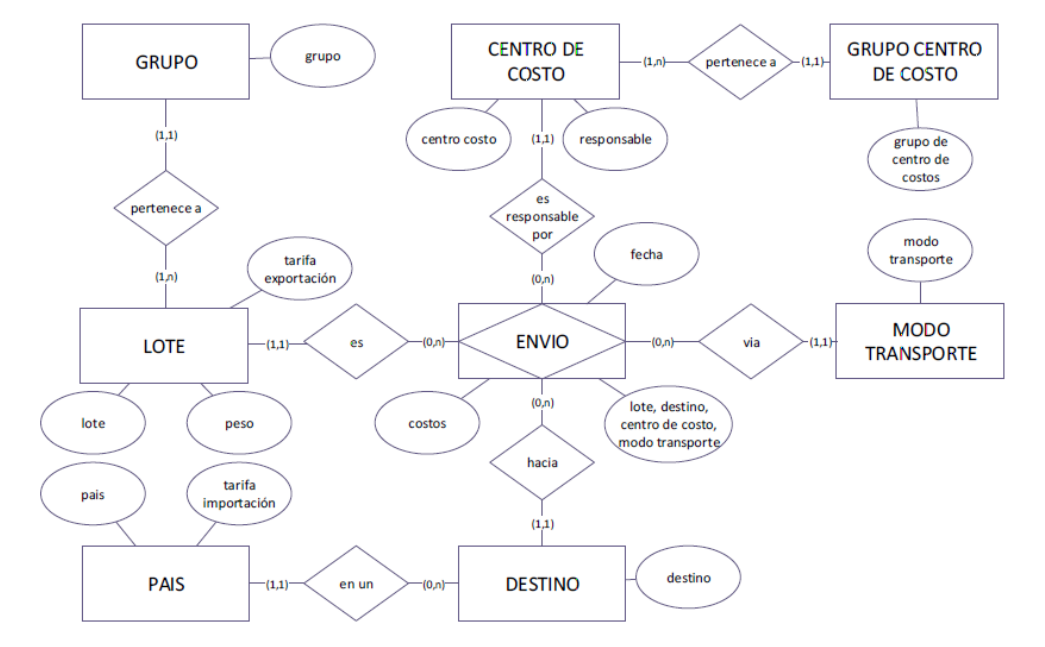
\includegraphics[width=12cm]{./Imagenes/MODELO_ER_1} 
\end{center}

Supongamos que los costos de los atributos ya incluyen todas las tarifas. No se transferirá más información sobre las tarifas
al almacén de datos. El análisis tendrá lugar a nivel del grupo de centros de costos, no se necesita información sobre los
centros de costos.
Por favor identifique el hecho de interés y construya el Modelo Dimensional 


\begin{center}
	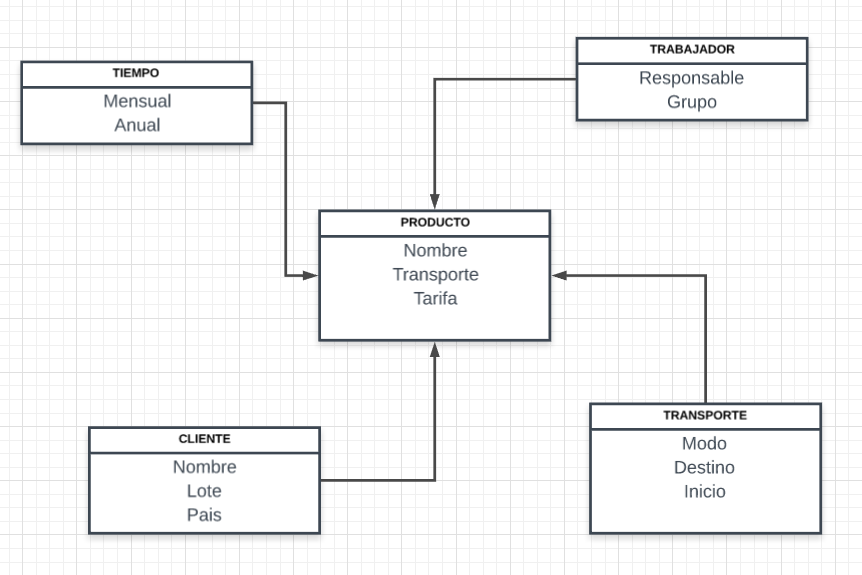
\includegraphics[width=12cm]{./Imagenes/MODELO_D_1} 
\end{center}


\item Ejercicio 02: Reservas de Viaje
En este esquema de E / R, un cliente (que es de cierto tipo) reserva un viaje en una agencia de viajes. La agencia de viajes
trabaja para un determinado operador turístico. El viaje va a un destino determinado que pertenece a un país determinado.
La dimensión de tiempo consiste en mes, trimestre y año

\begin{center}
	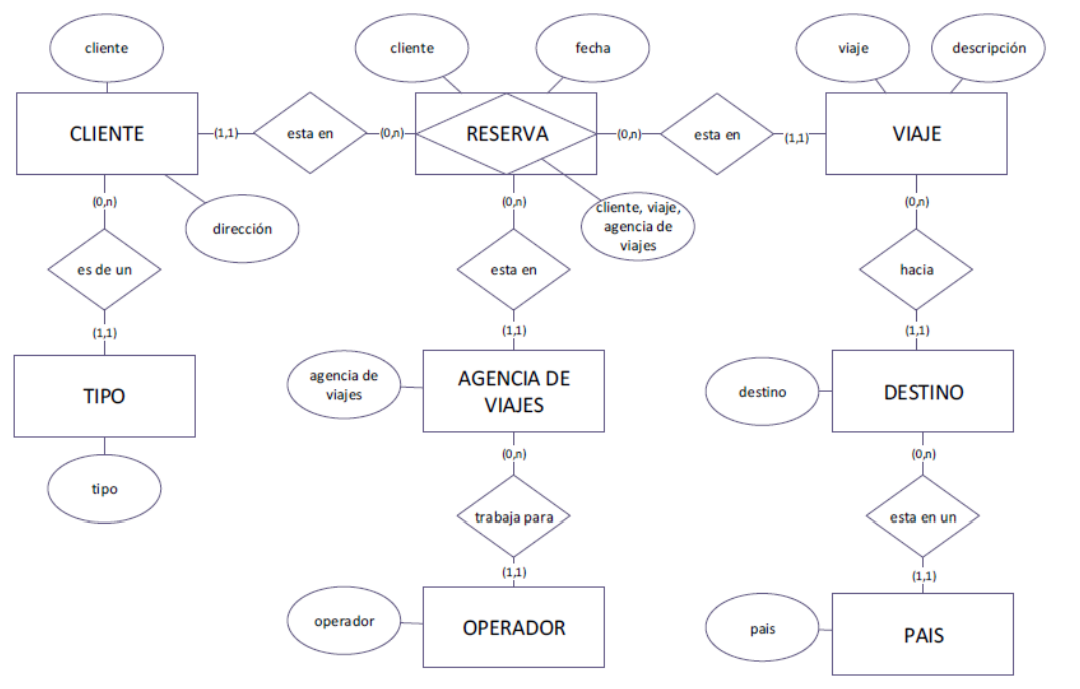
\includegraphics[width=12cm]{./Imagenes/MODELO_ER_2} 
\end{center}

Por favor identifique el hecho de interés y construya el Modelo Dimensional


\begin{center}
	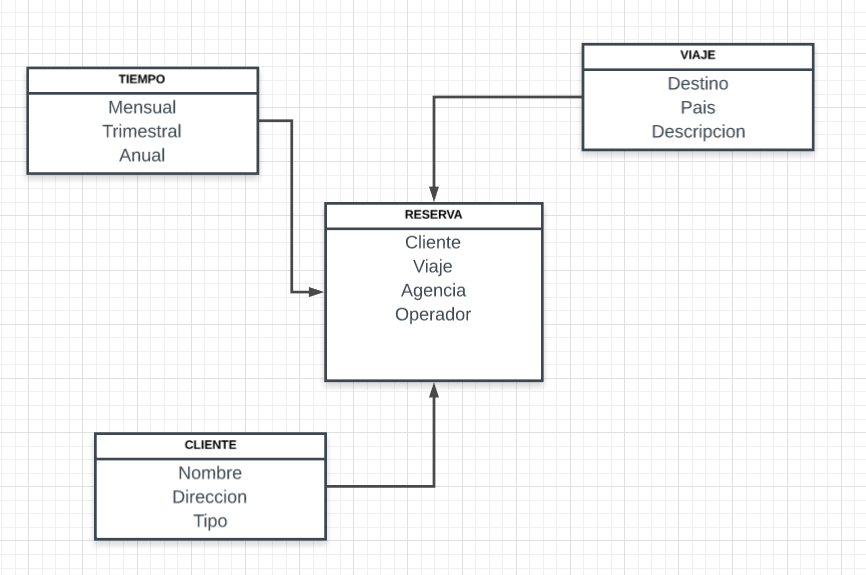
\includegraphics[width=12cm]{./Imagenes/MODELO_D_2} 
\end{center}


\item Ejercicio 03: Gestión de Proyectos 
Este esquema E / R simplificado muestra un caso gestión del proyecto.
El proyecto para un cliente se divide en varios paquetes de trabajo y siempre una persona es responsable de completar la
tarea. Se cuida en un lugar determinado.
La dimensión de tiempo consiste de día, mes y año


\begin{center}
	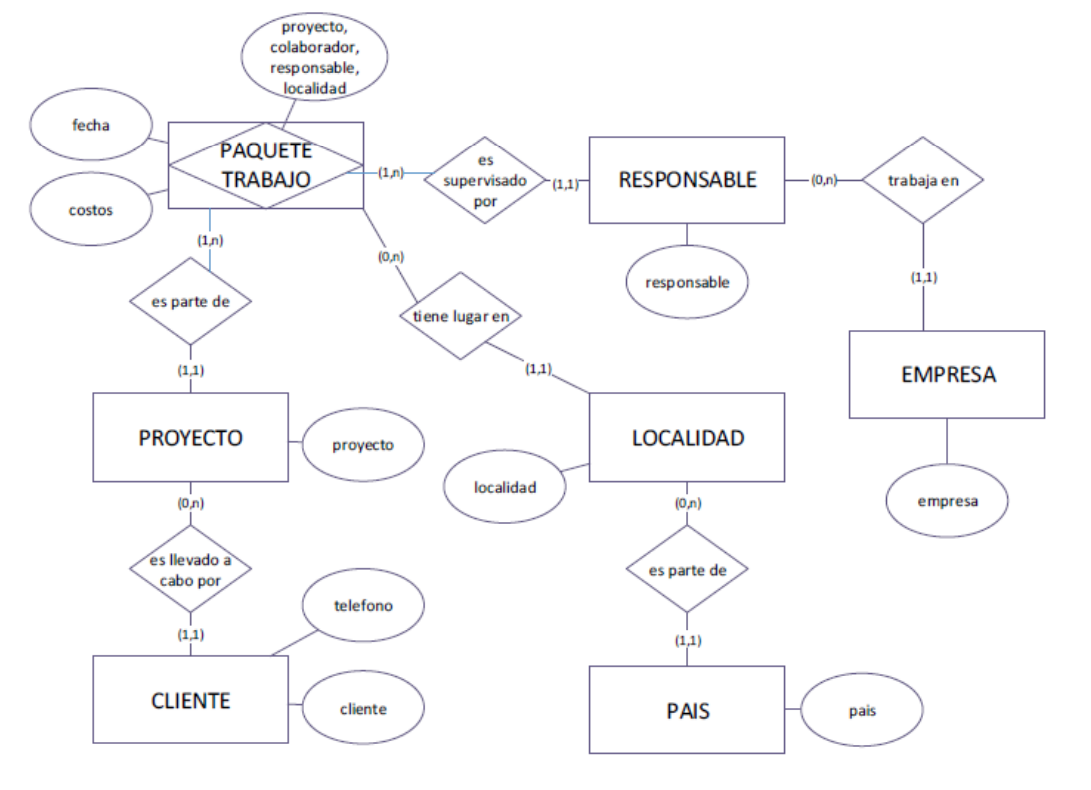
\includegraphics[width=12cm]{./Imagenes/MODELO_ER_3} 
\end{center}

Supongamos que los costos de los atributos ya incluyen todas las tarifas. No se transferirá más información sobre las tarifas
al almacén de datos. El análisis tendrá lugar a nivel del grupo de centros de costos, no se necesita información sobre los
centros de costos.
Por favor identifique el hecho de interés y construya el Modelo Dimensional 


\begin{center}
	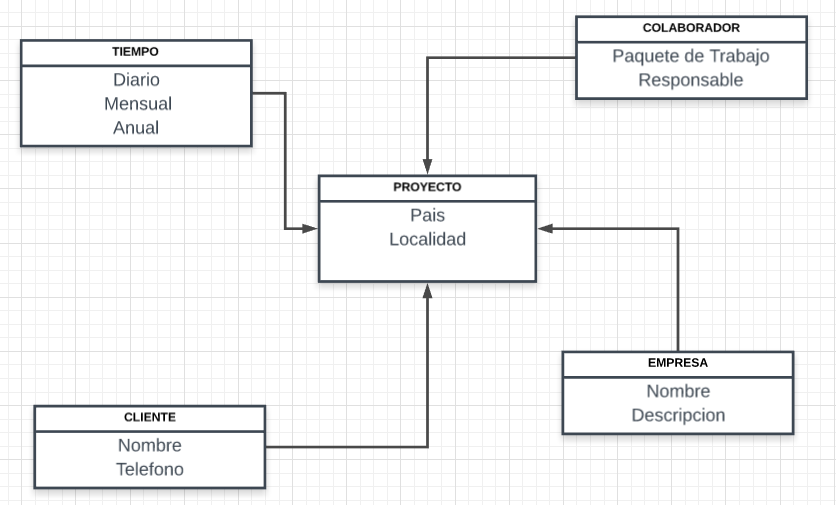
\includegraphics[width=12cm]{./Imagenes/MODELO_D_3} 
\end{center}

   
\end{itemize}


\section{Ventajas y Desventajas}

\subsection{Ventajas del Modelo Tabular}

\begin{itemize}
	\item Mucho más veloz en consultas.
	\item No requiere generar Aggregations (agregaciones) por lo que se simplifica el tiempo de procesamiento.
	\item Gracias al DAX (el lenguaje para acceder a los datos equivalente al MDX), tiene mayor flexibilidad para obtener información.
	\item Es intuitivo por lo que es mucho más rápido y fácil de entender e implementar.
	\item Se basa en modelos relacionales.
\end{itemize}

\subsection{Desventajas del Modelo Tabular}

\begin{itemize}
	\item Las particiones no se procesaban en paralelo si no secuencialmente, lo que hace que sea más lento el procesamiento.
	\item No se pueden usar multiples idiomas.
	\item Si son muchos datos tarda bastante en manejar configuraciones de diferentes particiones.
	\item El modelo tabular acapara demasiada memoria RAM y a su vez es dependiente de tal que afectará a otras aplicaciones.
\end{itemize}


\section{Diferencias}

\subsection{¿Qué modelo de datos utilizar? }

\section{Conclusiones}


\begin{itemize}
	\item Como conclusión Microsoft le está apuntando al modelo Tabular, puede consultar las mejoras de la próxima versión SQL 2016. En SQL 2012 y 2014 el modelo Tabular es bueno para BI pequeños y medianos volúmenes, para altos volúmenes es preferible el modelo Multidimensional.
	\item Power View proporciona informes intuitivos adhoc para usuarios finales. 
	\item El modelo tabular no admite el procesamiento paralelo de particiones, lo que puede tener un impacto significativo en el tiempo de procesamiento.
	\item Microsoft realmente sabe cómo lidiar con los requisitos del usuario y sabe que faltaba un puente entre el modelo de base de datos de relaciones y el modelo MOLAP. 
	\item Al introducir el motor xVelocity en SSAS y el modelo tabular incorporado, Microsoft proporciona herramientas de acceso al usuario que proporcionan una mejor solución con buena velocidad y rendimiento. 
\end{itemize}

%%
	
	%%
	%\linenumbers
	
	%% main text

	
	\newpage
	
		%ESTILO
	%ARCHIVO .bib
	   \begin{thebibliography}{0}

                 \bibitem{} https://www.element61.be/en/resource/choice-between-tabular-or-multidimensional-models-sql-server-analysis-services-2012
                  \bibitem{} https://docs.microsoft.com/es-es/sql/analysis-services/comparing-tabular-and-multidimensional-solutions-ssas?view=sql-server-2017
                    \bibitem{Brandon} https://www.businessintelligence.info/definiciones/que-es-modelo-dimensional.html


         \end{thebibliography}
	
\end{document}

%%
%% End of file `elsarticle-template-1-num.tex'.
